{\large\section*{Теоритические вопросы}}

\begin{enumerate}
	\item \textit{Что такое рекурсия? Как организуется хвостовая рекурсия в Prolog? Как организовать выход из рекурсии в Prolog?}

	\qquad \textbf{Ответ}: Рекурсия -- это один из способов организации повторных вычислений. Т.к. логическое программирование -- не операторное, то рекурсия -- это способ заставить систему использовать многократно одну и ту же процедуру. Хвостовая рекурсия в прологе организуется с помощью использования в определении знания того же знания.

	\item \textit{Какое первое состояние резольвенты?}
	
	\qquad \textbf{Ответ}: первое состояние резольвенты представляет собой вопрос.

	\item \textit{В каком случае система запускает алгоритм унификации? Каково назначение использования алгоритма унификации? Каков результат работы алгоритма унификации?}

	\qquad \textbf{Ответ}: алгоритм унификации запускается системой в случае необходимости проверить, подходит ли текущее правило в базе знаний для доказательства текущей цели. Результат алгоритма унификации представляет ответ да или нет. При ответе да результатом также является подстановка, сформированная в процессе работы алгоритма.
	
	\item \textit{В каких пределах программы уникальны переменные?}
	
	\qquad \textbf{Ответ}: именованные переменные уникальны в пределах предложения, а анонимные переменные уникальны всегда.

	\item \textit{Как применяется подстановка, полученная с помощью алгоритма унификации?}
	
	\qquad \textbf{Ответ}: все переменные, содержащиеся в постановке и в термах резольвенты, заменяются в резольвенте на соответствующие значения для этих переменных.

	\item \textit{Как изменяется резольвента?}
	
	\qquad \textbf{Ответ}: при нахождении похдодящего правила для первого терма резольвенты он заменяется на тело правила.
	
	\item \textit{В каких случаях запускается механизм отката?}

	\qquad \textbf{Ответ}: механизм отката запускается в случае, когда система попадает в тупиковое состояние -- резольвента не пуста, но вся база знаний уже была просмотрена с целью подбора знания для текущей цели доказательства.
\end{enumerate}

{\large\section*{Задание}}

Используя хвостовую рекурсию, разработать эффективную программу, (комментируя назначение аргументов), позволяющую:

\begin{enumerate}[1.]
	\item Найти длину списка (по верхнему уровню);
	\item Найти сумму элементов числового списка;
	\item Найти сумму элементов числового списка, стоящих на нечетных позициях исходного списка (нумерация от 0).
\end{enumerate}

Убедиться в правильности результатов.

Для одного из вариантов ВОПРОСА и каждого задания составить таблицу, отражающую конкретный порядок работы системы.

\clearpage

{\large\section*{Текст программы}}

\begin{lstlisting}
domains
	num = integer
	elemList = num*

predicates
	length(num, elemList).
	sum(num, elemList).
	sum_odd_id(num, elemList).

clauses
	length(0, []) :- !.
	length(R, [_|T]) :-
		length(R_1, T),
		R = R_1 + 1.
	
	sum(0, []) :- !.
	sum(R, [R]) :- !.
	sum(R, [H|T]) :-
		sum(R1, T),
		R = H + R1.
	
	sum_odd_id(0, []) :- !.
	sum_odd_id(0, [_]) :- !.
	sum_odd_id(R, [_, R]) :- !.
	sum_odd_id(R, [_, H|T]) :-
		sum_odd_id(R1, T),
		R = R1 + H.

goal
	sum_odd_id(R, [1, 2, 3, 4, 5]).
\end{lstlisting}

\clearpage

{\large\section*{Порядок поиска ответа для вопросов}}

Порядок поиска ответа для вопроса: \texttt{length(R, [2, 1, 5])}

\vspace*{5mm}

\begin{center}
	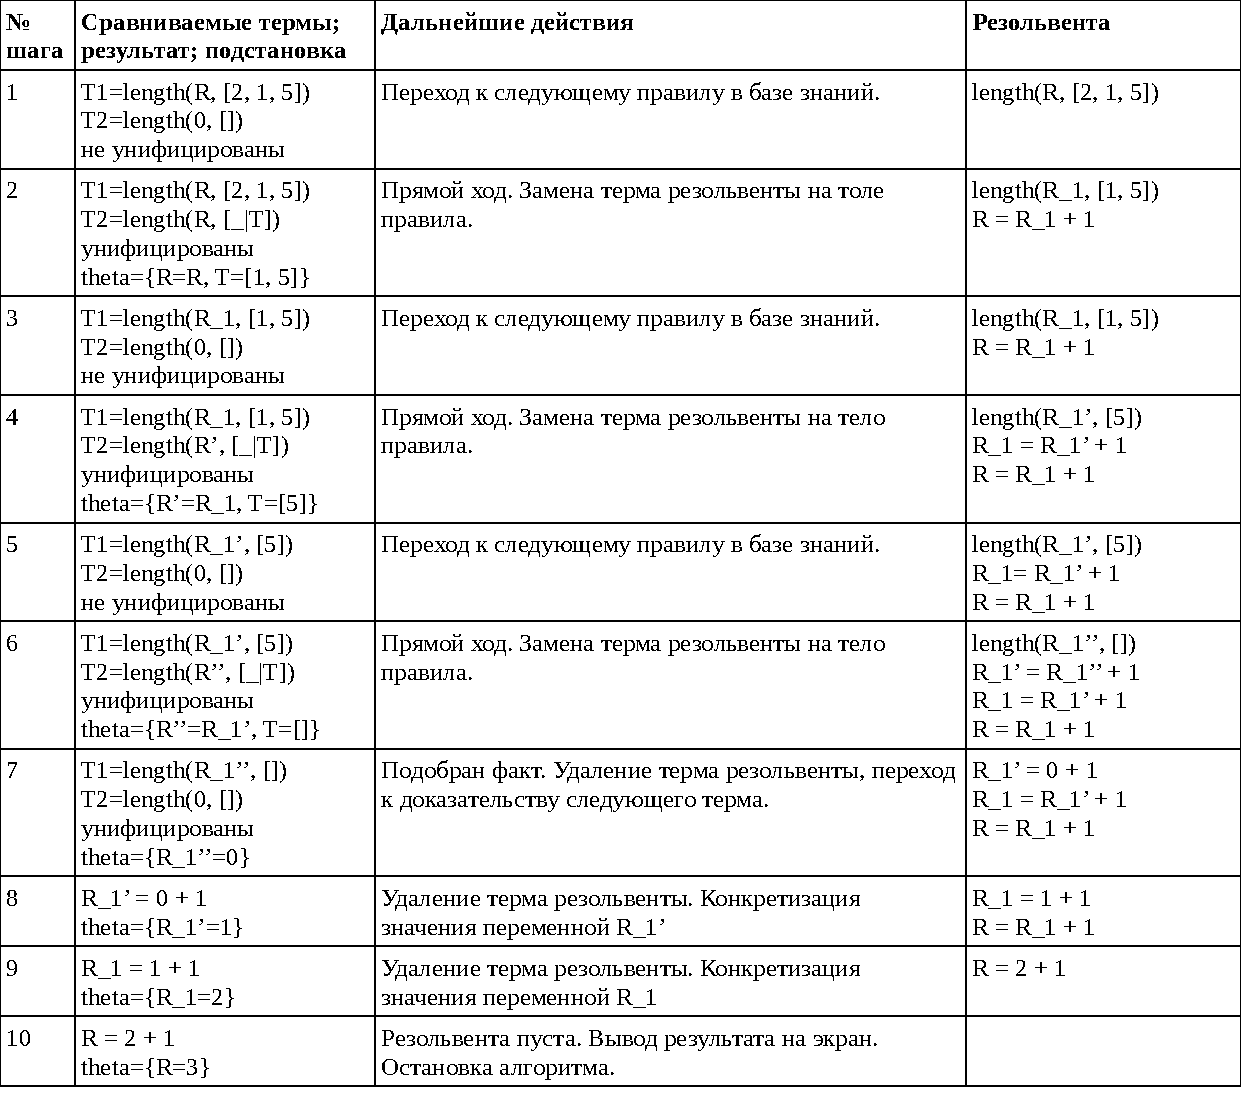
\includegraphics[width=\linewidth]{table1.pdf}
\end{center}

% Порядок поиска ответа для 2 варианта:

%\begin{center}
%	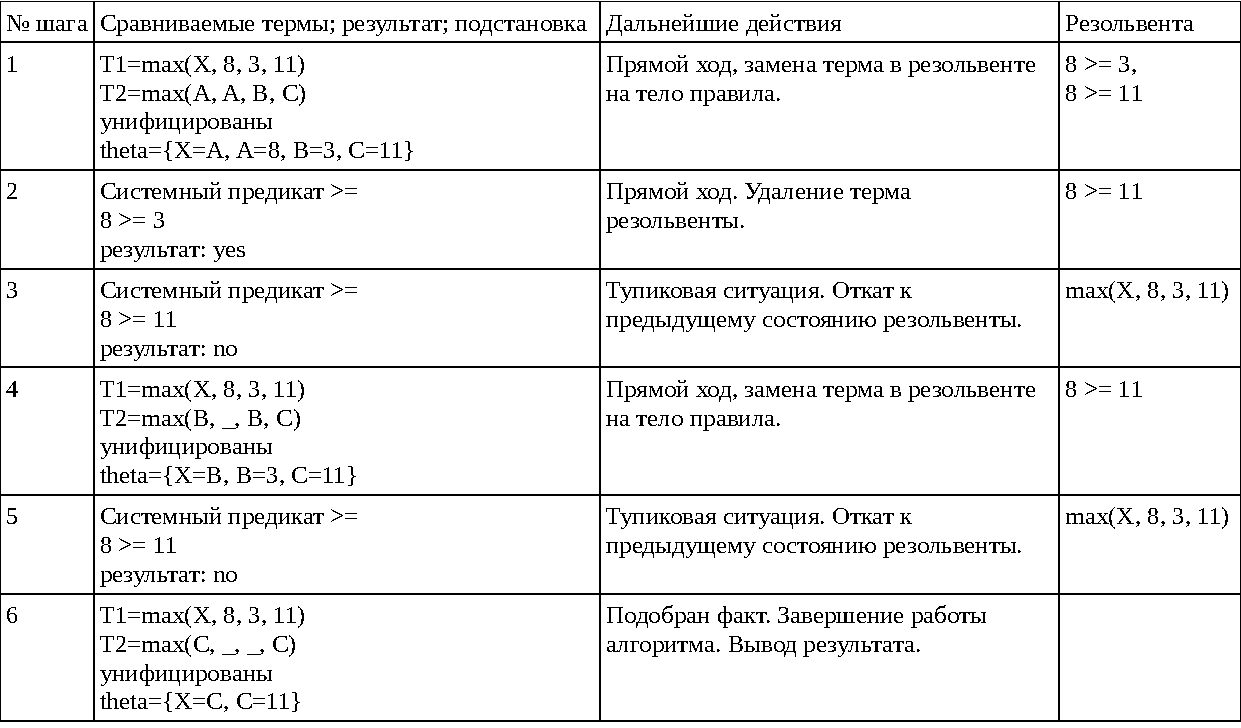
\includegraphics[width=\linewidth]{table2.pdf}
%\end{center}
